\documentclass[12pt, openany, oneside]{book}

\usepackage{listings}
\usepackage[dvipsnames]{xcolor}
\usepackage{ctex}
\usepackage{fontspec}
\usepackage{setspace}
\usepackage{tikz}
\usepackage{anyfontsize}
\usepackage{sectsty}
\usepackage{titlesec}
\usepackage{float}
\usepackage[hidelinks]{hyperref}
\usepackage[a4paper]{geometry}
\usepackage{url}
\usepackage{amssymb}
\usepackage{fontawesome5}
\usepackage[most]{tcolorbox}
\usepackage{circuitikz}
\usepackage{stackengine}
\usepackage{multirow}
\usepackage{newtxtt}
% \usepackage{minted}

\makeatletter
\newcommand{\verbatimfont}[1]{\renewcommand{\verbatim@font}{\ttfamily#1}}
\makeatother

\usetikzlibrary{calc,trees,positioning,arrows,fit,shapes}
\usetikzlibrary{shapes.multipart,chains}
\usetikzlibrary{automata}

\usetikzlibrary{arrows,positioning, calc,lindenmayersystems,decorations.pathmorphing,intersections}
\tikzstyle{resource}= [draw,minimum size=30pt,inner sep=0pt]
\tikzstyle{process} = [draw,minimum size=30pt,inner sep=0pt,circle]
\tikzstyle{allocated} = [->,thick,arrows={-latex}]
\tikzstyle{requested} = [<-,thick,arrows={latex-}, dashed]

\def\rlwd{.5pt} \def\rlht{2.2ex} \def\rldp{.5ex}
\def\mydiv#1{~%
  \rule[-\rldp]{\rlwd}{\rlht}%
  \setbox0=\hbox{~#1}%
  \stackunder[\dimexpr\rldp-\rlwd]{~#1}{\rule{\wd0}{\rlwd}}%
}

\definecolor{mycolor}{RGB}{0,128,128}
\newtcbox{\mybox} {
    on line,
    colback=mycolor,
    fontupper=\bfseries\color{white},
    boxrule=0pt,
    arc=5pt, 
    boxsep=0pt, 
    left=2pt, 
    right=2pt, 
    top=5pt, 
    bottom=5pt
}

\setstretch{1.5}
\setlength{\parindent}{0cm}

\geometry{a4paper,top=2.5cm,bottom=2.5cm}

\titleformat{\chapter}{\Huge\Huge\bfseries}{\chaptertitlename\ \thechapter{\ }}{0pt}{\Huge}{}
\titlespacing{\chapter}{0pt}{0pt}{12pt}

\definecolor{dkgreen}{rgb}{0,0.4,0}
\definecolor{gray}{rgb}{0.5,0.5,0.5}
\definecolor{mauve}{rgb}{0.58,0,0.82}
\definecolor{LightGray}{gray}{0.9}

\lstset{
    basicstyle=\linespread{1.3} \fontspec{Consolas},    %  the size of the fonts that are used for the code
	basewidth=0.5em,
    numbers=left,            % where to put the line-numbers
    numberstyle=\color{black},  % the style that is used for the line-numbers
    numbersep=10pt,                  % how far the line-numbers are from the code
    backgroundcolor=\color{white},
    showspaces=false,
    showstringspaces=false,
    showtabs=false,
    frame=single,                   % adds a frame around the code
    rulecolor=\color{black},        % if not set, the frame-color may be changed on line-breaks within not-black text (e.g. commens (green here))
    tabsize=4,                      % sets default tabsize to 2 spaces
    captionpos=t,                   % sets the caption-position to bottom
    breaklines=false,                % sets automatic line breaking
    breakatwhitespace=true,        % sets if automatic breaks should only happen at whitespace
    title=\lstname,                   % show the filename of files included with \lstinputlisting;
    % also try caption instead of title
    numberstyle=\color{black},		% line number color
    keywordstyle=\color{blue},          % keyword style
    commentstyle=\color{dkgreen},       % comment style
    stringstyle=\color{mauve},         % string literal style
    escapeinside={\%*}{*)},            % if you want to add LaTeX within your code
    morekeywords={*,...}               % if you want to add more keywords to the set
}

\begin{document}

\thispagestyle{empty}

\begin{tikzpicture}[overlay,remember picture]
	% Background color
	\fill[
		black!2]
	(current page.south west) rectangle (current page.north east);

	% Rectangles
	\shade[
		left color=Dandelion,
		right color=Dandelion!40,
		transform canvas ={rotate around ={45:($(current page.north west)+(0,-6)$)}}]
	($(current page.north west)+(0,-6)$) rectangle ++(9,1.5);

	\shade[
		left color=lightgray,
		right color=lightgray!50,
		rounded corners=0.75cm,
		transform canvas ={rotate around ={45:($(current page.north west)+(.5,-10)$)}}]
	($(current page.north west)+(0.5,-10)$) rectangle ++(15,1.5);

	\shade[
		left color=lightgray,
		rounded corners=0.3cm,
		transform canvas ={rotate around ={45:($(current page.north west)+(.5,-10)$)}}] ($(current page.north west)+(1.5,-9.55)$) rectangle ++(7,.6);

	\shade[
		left color=orange!80,
		right color=orange!60,
		rounded corners=0.4cm,
		transform canvas ={rotate around ={45:($(current page.north)+(-1.5,-3)$)}}]
	($(current page.north)+(-1.5,-3)$) rectangle ++(9,0.8);

	\shade[
		left color=red!80,
		right color=red!80,
		rounded corners=0.9cm,
		transform canvas ={rotate around ={45:($(current page.north)+(-3,-8)$)}}] ($(current page.north)+(-3,-8)$) rectangle ++(15,1.8);

	\shade[
		left color=orange,
		right color=Dandelion,
		rounded corners=0.9cm,
		transform canvas ={rotate around ={45:($(current page.north west)+(4,-15.5)$)}}]
	($(current page.north west)+(4,-15.5)$) rectangle ++(30,1.8);

	\shade[
		left color=RoyalBlue,
		right color=Emerald,
		rounded corners=0.75cm,
		transform canvas ={rotate around ={45:($(current page.north west)+(13,-10)$)}}]
	($(current page.north west)+(13,-10)$) rectangle ++(15,1.5);

	\shade[
		left color=lightgray,
		rounded corners=0.3cm,
		transform canvas ={rotate around ={45:($(current page.north west)+(18,-8)$)}}]
	($(current page.north west)+(18,-8)$) rectangle ++(15,0.6);

	\shade[
		left color=lightgray,
		rounded corners=0.4cm,
		transform canvas ={rotate around ={45:($(current page.north west)+(19,-5.65)$)}}]
	($(current page.north west)+(19,-5.65)$) rectangle ++(15,0.8);

	\shade[
		left color=OrangeRed,
		right color=red!80,
		rounded corners=0.6cm,
		transform canvas ={rotate around ={45:($(current page.north west)+(20,-9)$)}}]
	($(current page.north west)+(20,-9)$) rectangle ++(14,1.2);

	% Year
	% \draw[ultra thick,gray]
	% ($(current page.center)+(5,2)$) -- ++(0,-3cm)
	node[
			midway,
			left=0.25cm,
			text width=5cm,
			align=right,
			black!75
		]
		{
			% {\fontsize{25}{30} \selectfont \bf ANNUAL \\[10pt] REPORT}
		}
	node[
			midway,
			right=0.25cm,
			text width=6cm,
			align=left,
			orange]
		{
			% {\fontsize{72}{86.4} \selectfont 2020}
		};

	% Title
	\node[align=center] at ($(current page.center)+(0,-7)$)
	{
	{\fontsize{72}{72} \selectfont {{数据库}}} \\[1cm]
	{\fontsize{42}{42} \selectfont {{Database}}} \\[2cm]
	{\fontsize{20}{19.2} \selectfont \textcolor{orange}{ \bf 极夜酱}} \\[4pt]
	};
\end{tikzpicture}

\newpage

\pagestyle{plain}
\setcounter{page}{1}
\setcounter{tocdepth}{0}
\tableofcontents

\newpage

\setcounter{page}{1}

% \chapter{数据库简介}

% \section{数据库(Database)}

% 当今的程序开发几乎都是围绕着数据库展开的,一个合理且通用的程序一定要有数据库的开发支持。 \\

% 数据库的产生最初是由IBM的一个分析人员在70年代推出的《论关系型数据库的发展》论文开始的。这篇论文一公布之后,全世界就出现了几十种不同的数据库,其中到现在还能够继续存在的数据库是Oracle,而其它的数据库要么被收购了,要么就是彻底消失了。后来IBM为了统一数据库操作,后来又推出了SQL语法结构,并且该结构也已经成为当今数据库的使用标准。

% \section{SQL(Structured Query Language)}

% SQL是一种结构化查询语言,用于数据库的访问,自1970年代诞生到现在,经久不衰,日久弥新。数据库早已遍布各个应用领域,数据管理、数据分析甚至机器学习都可以用SQL来完成。 \\

% SQL可用于在数据库中增加、删除、修改、查询数据,用于简单的数据清洗和数据分析,并可搭配其它工具制作数据报表、大数据和机器学习。 \\

% 关系数据库管理系统RDBMS(Relational Database Management System)是一种数据库软件,它将数据和数据关系以数据库和数据表的形式存储,并提供SQL访问接口。目前主流的RDBMS有MySQL、PostgreSQL、SQL Server和Oracle,其中MySQL和PostgreSQL是免费开源且使用广泛的数据库。 \\

% SQL的关键字不区分大小写,如CREATE和create的作用相同,但推荐关键字大写。SQL语句中如果包含保留词需要通过转义符转义,例如MySQL中的转义符是反引号。

% SQL是是用来操作数据的基本单位,每一条SQL语句末尾必须有分号。 \\

% SQL可以分为数据操作语言DML(Data Manipulation Language)和数据定义语言DDL(Data Definition Language)。 \\

% DDL负责数据结构定义和数据库对象定义,主要由CREATE、ALTER、DROP三个指令组成:

% \begin{table}[H]
% 	\centering
% 	\setlength{\tabcolsep}{5mm}{
% 		\begin{tabular}{|c|c|}
% 			\hline
% 			\textbf{指令}   & \textbf{功能} \\
% 			\hline
% 			CREATE DATABASE & 创建数据库    \\
% 			\hline
% 			ALTER DATABASE  & 修改数据库    \\
% 			\hline
% 			CREATE TABLE    & 创建数据表    \\
% 			\hline
% 			ALTER TABLE     & 修改数据表    \\
% 			\hline
% 			DROP DATABASE   & 删除数据库    \\
% 			\hline
% 			DROP TABLE      & 删除数据表    \\
% 			\hline
% 		\end{tabular}
% 	}
% 	\caption{DDL指令}
% \end{table}

% DML负责数据访问和数据操作,主要由INSERT、DELETE、SELECT、UPDATE组成:

% \begin{table}[H]
% 	\centering
% 	\setlength{\tabcolsep}{5mm}{
% 		\begin{tabular}{|c|c|}
% 			\hline
% 			\textbf{指令} & \textbf{功能} \\
% 			\hline
% 			SELECT FROM   & 查询数据      \\
% 			\hline
% 			UPDATE SET    & 更新数据      \\
% 			\hline
% 			DELETE FROM   & 删除数据      \\
% 			\hline
% 			INSERT INTO   & 新增数据      \\
% 			\hline
% 		\end{tabular}
% 	}
% 	\caption{DML指令}
% \end{table}

% \section{数据类型}

% 数据库之中最基本的数据管理单位是数据表,每一个数据表中会存在若干个数据列,每一种数据列都有各自对应的数据类型。 \\

% \begin{figure}[H]
% 	\centering
% 	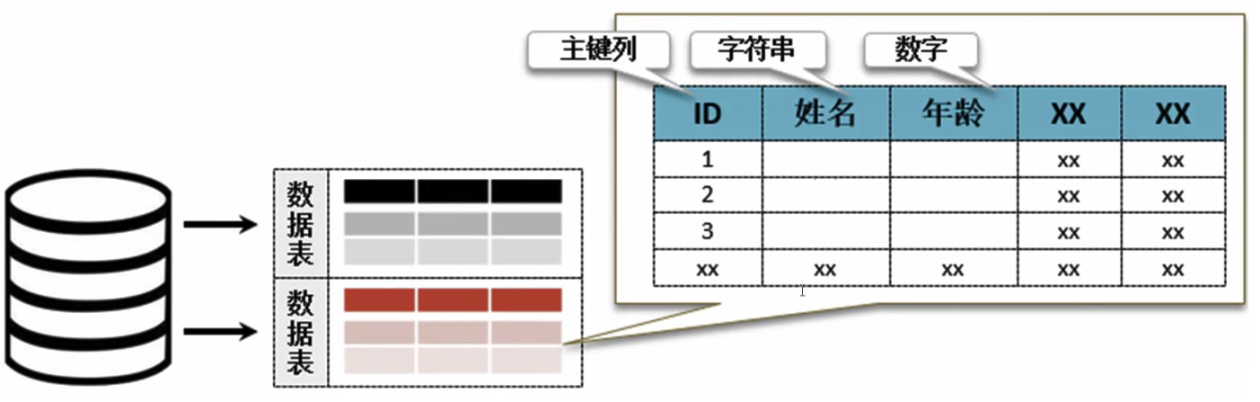
\includegraphics[]{img/C1/1.png}
% 	\caption{数据库}
% \end{figure}

% 数据表中的每个字段都需要明确地指明数据类型。常见的数据类型包括数值型、字符型和日期型。 \\

% 数值型分为整数类型和小数类型两类:

% \begin{enumerate}
% 	\item 整数类型默认有符号,无符号需要使用unsigned关键字约束,约束后不可表示负数。整数类型有数据长度的限制,如果在数据插入时超出其整型范围,数据库会报异常并插入失败。整数类型可以接受一个参数,表示它的最大显示宽度。

% 	\item 小数类型由整数部分和小数部分组成,指定时可以传入两个参数,分别表示整体的长度和小数部分的长度。
% \end{enumerate}

% \begin{table}[H]
% 	\centering
% 	\setlength{\tabcolsep}{5mm}{
% 		\begin{tabular}{|c|c|c|}
% 			\hline
% 			\textbf{数据类型} & \textbf{字节} & \textbf{描述} \\
% 			\hline
% 			tinyint(size)     & 1             & 极小整型      \\
% 			\hline
% 			smallint(size)    & 2             & 小整型        \\
% 			\hline
% 			mediumint(size)   & 3             & 中整型        \\
% 			\hline
% 			int(size)         & 4             & 整型          \\
% 			\hline
% 			bigint(size)      & 8             & 大整型        \\
% 			\hline
% 			float(size, d)    & 4             & 单精度浮点数  \\
% 			\hline
% 			double(size, d)   & 8             & 双精度浮点数  \\
% 			\hline
% 			decimal(size, d)  & 8             & 货币类型      \\
% 			\hline
% 			numeric(size, d)  & 8             & 同decimal     \\
% 			\hline
% 		\end{tabular}
% 	}
% 	\caption{数值型}
% \end{table}

% 字符类型表示文本和字符,根据字符串的长度,可以分为短文本和长文本两类。常见的短文本类型有char(不可变长)和varchar(可变长),长本文有text和blob,其中blob用来保存二进制流数据。

% \begin{table}[H]
% 	\centering
% 	\setlength{\tabcolsep}{5mm}{
% 		\begin{tabular}{|c|c|c|}
% 			\hline
% 			\textbf{数据类型} & \textbf{可否变长} & \textbf{描述}                \\
% 			\hline
% 			char(size)        & 不可              & 固定长度短字符串             \\
% 			\hline
% 			varchar(size)     & 可以              & 不固定长度短字符串           \\
% 			\hline
% 			text              & 可以              & 长字符串,保存文章内容       \\
% 			\hline
% 			blob              & 可以              & 二进制流,保存图片、媒体信息 \\
% 			\hline
% 		\end{tabular}
% 	}
% 	\caption{字符型}
% \end{table}

% \newpage

% \chapter{MySQL安装配置}

% \section{MySQL}

% MySQL是一款开源的关系型数据库,并且使用的人群众多,国内许多的开发公司为了节约软件开发成本,往往会使用大量免费开源的工具,所以MySQL这种小巧而且免费的数据库就非常受欢迎。随着MySQL版本的不断提升,很多的功能也在不断完善。 \\

% MySQL软件可直接通过官网\href{https://dev.mysql.com/downloads/mysql/8.0.html}进行下载。 \\

% \begin{figure}[H]
% 	\centering
% 	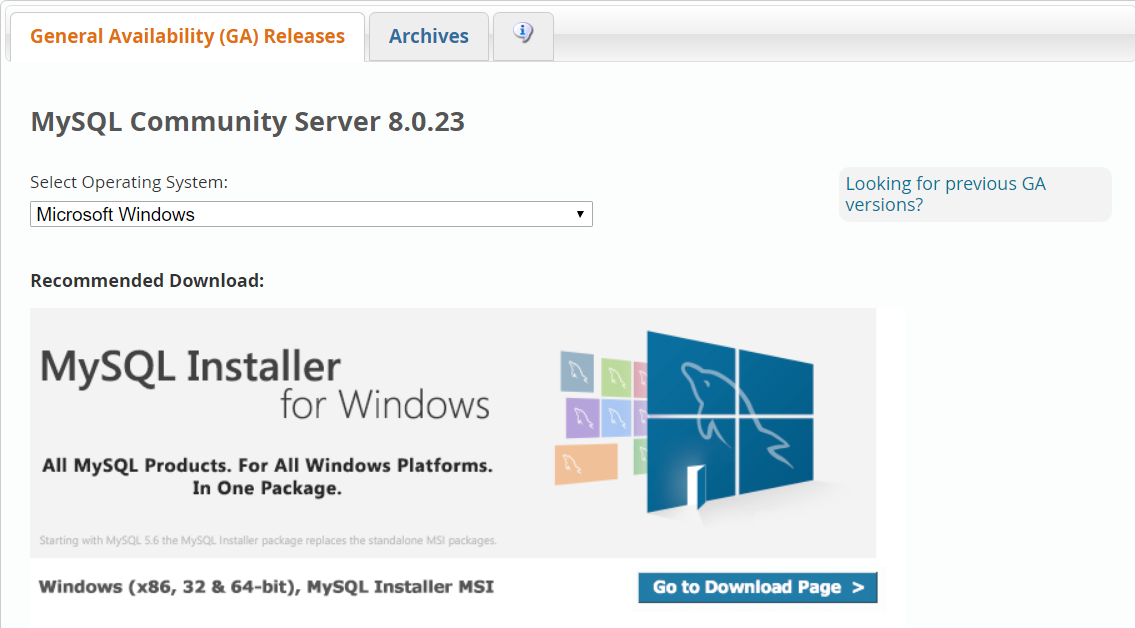
\includegraphics[scale=0.5]{img/C2/1.png}
% 	\caption{MySQL官网}
% \end{figure}

% 选择默认的Windows系统即可(尽量使用Win10系统安装,如果使用的是老系统往往需要安装大量的系统补丁)。 \\

% \begin{figure}[H]
% 	\centering
% 	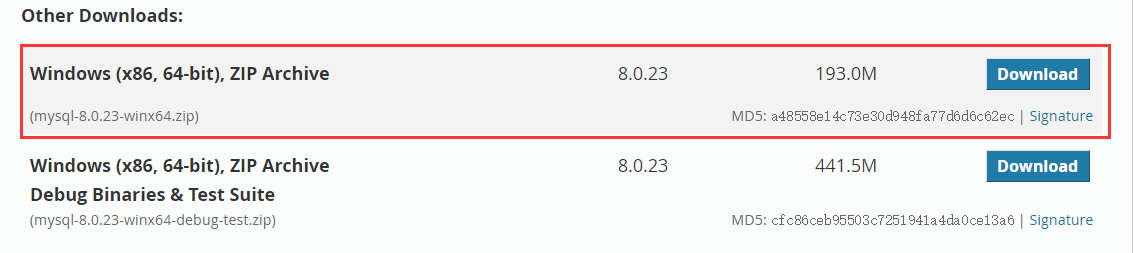
\includegraphics[scale=0.5]{img/C2/2.png}
% \end{figure}

% MySQL安装步骤:

% \subsubsection{解压缩}

% 建议将其解压缩到C盘根目录下,为了方便配置,将文件夹重命名为`mysql8`(完整路径:C:$ \backslash $mysql8)。

% \subsubsection{路径配置}

% 修改本地PATH环境属性,添加MySQL可执行文件路径。 \\

% \begin{figure}[H]
% 	\centering
% 	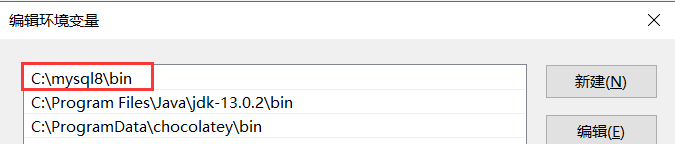
\includegraphics[]{img/C2/3.png}
% 	\caption{路径配置}
% \end{figure}

% \subsubsection{数据目录}

% MySQL所提供的仅仅是一个软件支持,但是数据库本身一定需要进行数据存储,就需要为其创建存储目录D:$ \backslash $mysql-dc$ \backslash $data和D:$ \backslash $mysql-dc$ \backslash $logs,其中data保存真实数据,logs保存相关日志。

% \subsubsection{MySQL配置}

% 通过配置文件my.ini建立C:$ \backslash $mysql8和D:$ \backslash $mysql-dc两个目录之间的联系。 \\

% \begin{figure}[H]
% 	\centering
% 	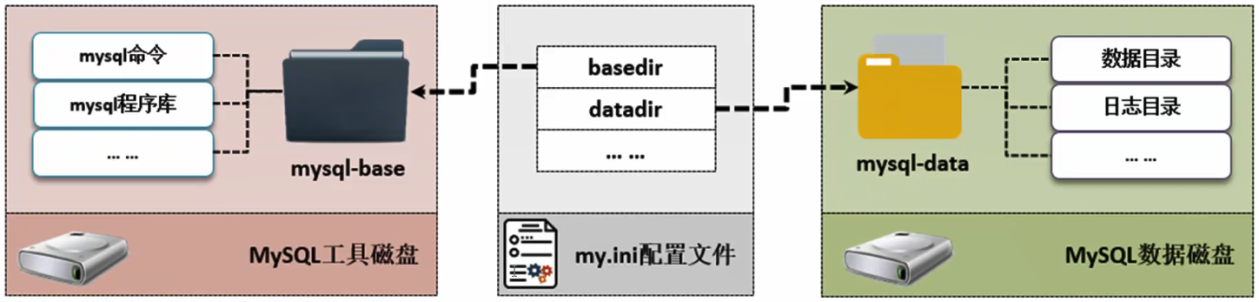
\includegraphics[]{img/C2/4.png}
% 	\caption{MySQL配置}
% \end{figure}

% \mybox{创建my.ini文件}

% \begin{lstlisting}
% [mysqld]
% # 设置3306端口
% port=3306
% # 设置mysql的安装目录
% basedir=C:\mysql8
% # 设置mysql数据库的数据的存放目录
% datadir=D:\mysql-dc\data
% # mysqlsock存储目录
% socket=D:\mysql-dc\data\mysql.sock
% # 允许最大连接数
% max_connections=10000
% # 允许连接失败的次数。这是为了防止有人从该主机试图攻击数据库系统
% max_connect_errors=10
% # 服务端使用的字符集默认为UTF8
% character-set-server=UTF8MB4
% # 创建新表时将使用的默认存储引擎
% default-storage-engine=INNODB
% # 默认使用"mysql_native_password"插件认证
% default_authentication_plugin=mysql_native_password
% [mysql]
% # 设置mysql客户端默认字符集
% default-character-set=UTF8MB4
% # mysqlsock存储目录
% socket=D:\mysql-dc\data\mysql.sock
% [client]
% # 设置mysql客户端连接服务端时默认使用的端口
% port=3306
% default-character-set=utf8
% [mysqld_safe]
% log-error=D:\mysql-dc\logs\mysql.log
% pid-file=D:\mysql-dc\logs\mysql.pid
% # mysqlsock存储目录
% socket=D:\mysql-dc\data\mysql.sock
% \end{lstlisting}

% \subsubsection{数据库初始化}

% 在命令行中通过MySQL提供的命令生成结构性文件,数据库初始化的时候会自动生成一个临时的密码,在没有修改之前只能通过此密码进行MySQL数据库的访问。 \\

% \mybox{数据库初始化}

% \begin{lstlisting}
% mysqld --initialize --console
% \end{lstlisting}

% \begin{tcolorbox}
% 	\mybox{临时密码}
% 	\begin{verbatim}
% ah+K3SB2,B(B
% 	\end{verbatim}
% \end{tcolorbox}

% \subsubsection{服务安装}

% 将MySQL启动命令添加到服务之中。在进行服务安装的时候一般都需要管理员的操作权限,所以一定要以管理员的身份打开命令行工具,否则会出现Install/Remove of the Service Denied!错误信息。 \\

% \mybox{安装并开启服务}

% \begin{lstlisting}
% mysqld install
% net start mysql
% \end{lstlisting}

% \subsubsection{服务登录}

% 通过命令行的模式进行MySQL数据库登录。第一次密码为系统初始化时生成的临时密码。 \\

% \mybox{MySQL登录}

% \begin{lstlisting}
% mysql -uroot -pah+K3SB2,B(B
% \end{lstlisting}

% \subsubsection{修改密码}

% 将临时密码修改为自己的密码,将root超级管理员的密码设置为mysqladmin。 \\

% \mybox{修改密码}

% \begin{lstlisting}[language=SQL]
% alter user 'root'@'localhost' IDENTIFIED WITH mysql_native_password
% BY 'mysqladmin';
% \end{lstlisting}

% \subsubsection{远程登录配置}

% 此时的root账户只能够在本地进行登录访问,所以需要开启远程访问配置。 \\

% \mybox{远程登录配置}

% \begin{lstlisting}[language=SQL]
% # 进入配置数据库
% use mysql
% # 设置远程访问
% update user set user.Host='%' where user.User='root';
% # 配置立即生效
% flush privileges;
% \end{lstlisting}

% MySQL数据库需要通过命令的模式来完成,要想使用MySQL数据库就必须通过用户名和密码进行数据库的登录。 \\

% \mybox{数据库登录}

% \begin{lstlisting}[language=SQL]
% mysql -uroot -pmysqladmin
% \end{lstlisting}

% 在一个数据库平台上会存在许多的数据库,通过SHOW DATABASES;可以查看当前环境下所有已经存在的数据库信息。 \\

% \mybox{查看数据库}

% \begin{lstlisting}[language=SQL]
% SHOW DATABASES;
% \end{lstlisting}

% \begin{tcolorbox}
% 	\mybox{运行结果}
% 	\begin{verbatim}
% +--------------------+
% | Database           |
% +--------------------+
% | information_schema |
% | mysql              |
% | performance_schema |
% | sys                |
% +--------------------+
% 	\end{verbatim}
% \end{tcolorbox}

% \newpage

% \chapter{CREATE}

% \section{创建数据库}

% CREATE负责数据库对象的创建,数据库、数据表、数据库索引、函数等都可以使用CREATE来创建。 \\

% 既然在一个平台上会有许多的数据库,那么在使用的时候就必须明确地确定好一个数据库,通过USE命令来进行数据库的使用切换。

% \vspace{-0.5cm}

% \begin{lstlisting}[language=SQL]
% CREATE DATABASE [database_name];
% USE [database_name];
% \end{lstlisting}

% \vspace{0.5cm}

% \mybox{创建student数据库}

% \begin{lstlisting}[language=SQL]
% CREATE DATABASE student;
% USE student;
% \end{lstlisting}

% SQL语句可以保存到.sql脚本中,在连接MySQL数据库后使用source指定脚本路径。

% \vspace{-0.5cm}

% \begin{lstlisting}[language=SQL]
% source [path]
% \end{lstlisting}

% \section{创建数据表}

% CREATE TABLE指令可以在数据库中创建数据表。通过DESC指令可以查看数据表结构。

% \vspace{-0.5cm}

% \begin{lstlisting}[language=SQL]
% CREATE TABLE [table_name](
%     [col1] [datatype1],
%     [col2] [datatype2],
%     [col3] [datatype3],
%     ....
% );

% DESC [table_name];
% \end{lstlisting}

% \vspace{0.5cm}

% \mybox{创建数据表} \\

% 创建info数据表,字段包括id、name、gpa。

% \vspace{-0.5cm}

% \begin{lstlisting}[language=SQL]
% CREATE TABLE info(
%     id int, 
%     name varchar(16), 
%     gpa double(5, 2)
% );

% DESC info;
% \end{lstlisting}

% \begin{tcolorbox}
% 	\mybox{运行结果}
% 	\begin{verbatim}
% +-------+-------------+------+-----+---------+-------+
% | Field | Type        | Null | Key | Default | Extra |
% +-------+-------------+------+-----+---------+-------+
% | id    | int         | YES  |     | NULL    |       |
% | name  | varchar(16) | YES  |     | NULL    |       |
% | gpa   | double(5,2) | YES  |     | NULL    |       |
% +-------+-------------+------+-----+---------+-------+
% 	\end{verbatim}
% \end{tcolorbox}

% NULL是对未知/缺失属性的标识,常用于表示某个字段为空,NULL是所有可以为空字段的默认值。 \\

% NULL必须使用运算符IS和IS NOT进行比较。NULL与0并不是等价的,它们无法比较。

% \section{约束(Constraint)}

% SQL约束用于在新建或修改数据表时,给数据表或数据表中的字段加上约束条件。约束既可以在字段上,也可以在表上。一个字段,或者一张表可以有多个约束。

% \vspace{-0.5cm}

% \begin{lstlisting}[language=SQL]
% CREATE TABLE [table_name](
%     [col1] [datatype1] [constraint1],
%     [col2] [datatype2] [constraint2],
%     [col3] [datatype3] [constraint3],
%     ....,
%     [constraint4]
% );
% \end{lstlisting}

% \begin{table}[H]
% 	\centering
% 	\setlength{\tabcolsep}{5mm}{
% 		\begin{tabular}{|c|c|}
% 			\hline
% 			\textbf{约束} & \textbf{功能} \\
% 			\hline
% 			NOT NULL      & 字段非空      \\
% 			\hline
% 			DEFAULT       & 字段默认值    \\
% 			\hline
% 			UNIQUE        & 字段唯一      \\
% 			\hline
% 			PRIMARY KEY   & 主键          \\
% 			\hline
% 			FOREIGN KEY   & 外键          \\
% 			\hline
% 			CHECK         & 校验字段      \\
% 			\hline
% 		\end{tabular}
% 	}
% 	\caption{约束}
% \end{table}

% \begin{itemize}
% 	\item DEFAULT会给字段添加上默认值,若字段在添加的时候没有指定值,则使用默认值。

% 	\item NOT NULL表示一个字段是非空的,当在插入或者修改时,如果字段为空则报错。

% 	\item PRIMARY KEY表示主键,用于唯一标识数据表中的每一条记录。主键不能为空,并且必须是唯一的,即每条记录的主键必须各不相同。

% 	\item UNIQUE用于唯一数据表中的每一条记录,UNIQUE约束的字段必须是唯一的,即该字段在每条记录中必须各不相同。PRIMARY KEY约束默认拥有UNIQUE约束。每个表可以有多个UNIQUE约束,但是只能有一个PRIMARY KEY。
% \end{itemize}

% 在数据表已经存在的情况下不能重复创建同名表,因此需要使用DROP语句删除已经存在的数据表。 \\

% \mybox{约束} \\

% 创建info数据表,字段包括id、name、gpa,其中id为主键,name为非空字段,gpa默认为0。

% \vspace{-0.5cm}

% \begin{lstlisting}[language=SQL]
% DROP TABLE IF EXISTS info;

% CREATE TABLE info(
%     id int PRIMARY KEY,
%     name varchar(16) NOT NULL,
%     gpa double(5, 2) DEFAULT 0
% );

% DESC info;
% \end{lstlisting}

% \begin{tcolorbox}
% 	\mybox{运行结果}
% 	\begin{verbatim}
% +-------+-------------+------+-----+---------+-------+
% | Field | Type        | Null | Key | Default | Extra |
% +-------+-------------+------+-----+---------+-------+
% | id    | int         | NO   | PRI | NULL    |       |
% | name  | varchar(16) | NO   |     | NULL    |       |
% | gpa   | double(5,2) | YES  |     | 0.00    |       |
% +-------+-------------+------+-----+---------+-------+
%     \end{verbatim}
% \end{tcolorbox}

% \section{CHECK}

% CHECK约束用于限制字段值的范围,既可以定义在单个字段上,也可以在定义在表上对特定字段进行约束。CHECK可以在数据库层面上筛选掉不符合约束的数据。创建成功后,若插入的数据不满足条件,会导致插入失败。 \\

% \mybox{CHECK} \\

% 创建数据表info,包括id、name、age三个,age字段添加CHECK约束,规定所有age必须大于0。

% \vspace{-0.5cm}

% \begin{lstlisting}[language=SQL]
% DROP TABLE IF EXISTS info;

% CREATE TABLE info(
%     id int,
%     name varchar(20),
%     age int unsigned CHECK(age > 0)
% );

% DESC info;
% \end{lstlisting}

% \begin{tcolorbox}
% 	\mybox{运行结果}
% 	\begin{verbatim}
% +-------+--------------+------+-----+---------+-------+
% | Field | Type         | Null | Key | Default | Extra |
% +-------+--------------+------+-----+---------+-------+
% | id    | int          | YES  |     | NULL    |       |
% | name  | varchar(20)  | YES  |     | NULL    |       |
% | age   | int unsigned | YES  |     | NULL    |       |
% +-------+--------------+------+-----+---------+-------+
%     \end{verbatim}
% \end{tcolorbox}

% \newpage

% \chapter{ALTER}

% \section{初始数据}

% \mybox{初始数据}

% \begin{lstlisting}[language=SQL]
% DROP TABLE IF EXISTS info;

% CREATE TABLE info(
%     id int, 
%     name varchar(16), 
%     gpa double(5, 2)
% );
% \end{lstlisting}

% \section{ALTER}

% ALTER指令用于已有数据表的修改,增加、修改和删除数据表字段都可以通过ALTER来完成。ALTER使用户可以修改已创建的数据表,但大多数情况下数据表字段和类型需要在定义的时候就确认,ALTER修改数据表是非常消耗性能和时间的。 \\

% 添加、删除、修改字段语法如下:

% \vspace{-0.5cm}

% \begin{lstlisting}[language=SQL]
% ALTER TABLE [table_name] ADD ([col] [datatype]);
% ALTER TABLE [table_name] DROP [col];
% ALTER TABLE [table_name] MODIFY (COLUMN [col] [datatype] [constraint]);
% \end{lstlisting}

% \vspace{0.5cm}

% \mybox{ALTER} \\

% 为info表添加字段phone,类型为varchar(20);删除字段gpa;修改字段id类型为varchar(10),字段非空。

% \vspace{-0.5cm}

% \begin{lstlisting}[language=SQL]
% ALTER TABLE info ADD phone varchar(20);
% ALTER TABLE info DROP gpa;
% ALTER TABLE info MODIFY id varchar(10) NOT NULL;
% DESC info;
% \end{lstlisting}

% \begin{tcolorbox}
% 	\mybox{运行结果}
% 	\begin{verbatim}
% +-------+-------------+------+-----+---------+-------+
% | Field | Type        | Null | Key | Default | Extra |
% +-------+-------------+------+-----+---------+-------+
% | id    | varchar(10) | NO   |     | NULL    |       |
% | name  | varchar(16) | YES  |     | NULL    |       |
% | phone | varchar(20) | YES  |     | NULL    |       |
% +-------+-------------+------+-----+---------+-------+
%     \end{verbatim}
% \end{tcolorbox}

% \newpage

% \chapter{DROP}

% \section{DROP}

% DROP指令用于删除数据库、数据表、索引和视图等,DROP强大而又危险,它能迅速清理掉数据库垃圾,不过使用之前请仔细斟酌,删除的数据很可能再也找不回来了。DROP几乎可以清理掉数据库中的任何对象,因此在操作之前必须确保数据的安全性。 \\

% 删除数据库、诉苦表语法如下:

% \vspace{-0.5cm}

% \begin{lstlisting}[language=SQL]
% DROP DATABASE [db_name];
% DROP TABLE [table_name];
% \end{lstlisting}

% TRUNCATE指令可以在保留数据表的情况下清空数据表数据。

% \vspace{-0.5cm}

% \begin{lstlisting}[language=SQL]
% TRUNCATE TABLE [table_name];
% \end{lstlisting}

% \newpage

% \chapter{INSERT}

% \section{初始数据}

% \mybox{初始数据}

% \begin{lstlisting}[language=SQL]
% DROP TABLE IF EXISTS info;

% CREATE TABLE info(
%     id int,
%     name varchar(16),
%     gpa double(5, 2)
% );
% \end{lstlisting}

% \section{INSERT}

% INSERT指令用于向数据表中添加记录,INSERT插入数据分为普通插入和批量插入。并不是每个RDBMS都支持批量插入,批量插入的移植性并不好,如果所使用的数据库不支持,可以将其改为多个普通插入。

% \vspace{-0.5cm}

% \begin{lstlisting}[language=SQL]
% INSERT INTO [table_name] ([col1], [col2]) VALUES([val1], [val2]);
% \end{lstlisting}

% 如果插入的数据是全字段,那么可以省略前面的col。

% \vspace{-0.5cm}

% \begin{lstlisting}[language=SQL]
% INSERT INTO [table_name] VALUES([val1], [val2]);
% \end{lstlisting}

% \vspace{0.5cm}

% \mybox{单条插入} \\

% 向数据表info中插入一条记录,id为1,name为Terry,gpa为3.7。

% \vspace{-0.5cm}

% \begin{lstlisting}[language=SQL]
% INSERT INTO info VALUES(1, "Terry", 3.7);
% SELECT * FROM info;
% \end{lstlisting}

% \begin{tcolorbox}
% 	\mybox{运行结果}
% 	\begin{verbatim}
% +------+-------+------+
% | id   | name  | gpa  |
% +------+-------+------+
% |    1 | Terry | 3.70 |
% +------+-------+------+
%     \end{verbatim}
% \end{tcolorbox}

% 批量插入与普通插入的区别在于,VALUES关键字后面接受多个字段元组,每个()代表一个字段元组,一个字段元组会生成一条记录。

% \vspace{-0.5cm}

% \begin{lstlisting}[language=SQL]
% INSERT INTO [table_name] ([col1], [col2]) VALUES
% ([val1], [val2]),
% ([val1], [val2]);
% \end{lstlisting}

% \vspace{0.5cm}

% \mybox{批量插入} \\

% 向info表中插入两条记录,第一条记录\{2, "Lily", 4.2\},第二条记录\{3, "Eric", 3.3\}。

% \vspace{-0.5cm}

% \begin{lstlisting}[language=SQL]
% INSERT INTO info VALUES (2, "Lily", 4.2), (3, "Eric", 3.3);
% SELECT * FROM info;
% \end{lstlisting}

% \begin{tcolorbox}
% 	\mybox{运行结果}
% 	\begin{verbatim}
% +------+-------+------+
% | id   | name  | gpa  |
% +------+-------+------+
% |    1 | Terry | 3.70 |
% |    2 | Lily  | 4.20 |
% |    3 | Eric  | 3.30 |
% +------+-------+------+
%     \end{verbatim}
% \end{tcolorbox}

% \newpage

% \chapter{SELECT}

% \section{初始数据}

% \mybox{初始数据}

% \begin{lstlisting}[language=SQL]
% DROP TABLE IF EXISTS info;

% CREATE TABLE info(
%     id int,
%     name varchar(16),
%     gpa double(5, 2)
% );

% INSERT INTO info VALUES
% (1, "Terry", 3.7),
% (2, "Lily", 4.2),
% (3, "Eric", 3.3),
% (4, "Alice", 3.6),
% (5, "Lily", 4.2),
% (6, "Terry", 3.7),
% (7, "Anna", 4.1),
% (8, "Jason", 3.9);
% \end{lstlisting}

% \section{查询数据库信息}

% SELECT指令用于查询数据库中的数据,通过SELECT可以快速获取数据库中的变量和信息。 \\

% \mybox{查询数据库信息}

% \begin{lstlisting}[language=SQL]
% SELECT version();
% SELECT current_user;
% \end{lstlisting}

% \begin{tcolorbox}
% 	\mybox{运行结果}
% 	\begin{verbatim}
% +-----------+
% | version() |
% +-----------+
% | 8.0.26    |
% +-----------+

% +--------------+
% | current_user |
% +--------------+
% | root@%       |
% +--------------+
%     \end{verbatim}
% \end{tcolorbox}

% \section{查询数据表数据}

% 大部分情况下,SELECT都是用来获取数据表数据。

% \vspace{-0.5cm}

% \begin{lstlisting}[language=SQL]
% SELECT [col1], [col2] FROM [table_name];
% \end{lstlisting}

% SELECT后面跟的是要查询的字段名,若是查询所有字段,可以使用【*】表示。但是即使是获取全字段,也不推荐使用【*】,显式地给出查询字段,更容易维护和合作。

% \vspace{-0.5cm}

% \begin{lstlisting}[language=SQL]
% SELECT * FROM [table_name];
% \end{lstlisting}

% \vspace{0.5cm}

% \mybox{查询info表中name和gpa字段}

% \begin{lstlisting}[language=SQL]
% SELECT name, gpa FROM info;
% \end{lstlisting}

% \begin{tcolorbox}
% 	\mybox{运行结果}
% 	\begin{verbatim}
% +-------+------+
% | name  | gpa  |
% +-------+------+
% | Terry | 3.70 |
% | Lily  | 4.20 |
% | Eric  | 3.30 |
% | Alice | 3.60 |
% | Lily  | 4.20 |
% | Terry | 3.70 |
% | Anna  | 4.10 |
% | Jason | 3.90 |
% +-------+------+
%     \end{verbatim}
% \end{tcolorbox}

% 有时查询出来的所有数据会很多,SELECT在查询的时候可以使用LIMIT指定条数。

% \vspace{-0.5cm}

% \begin{lstlisting}[language=SQL]
% SELECT [col1], [col2] FROM [table_name] LIMIT n;
% \end{lstlisting}

% 有时想要查询指定起始位置指定条数的结果集,起始位置默认为0。

% \vspace{-0.5cm}

% \begin{lstlisting}[language=SQL]
% SELECT [col1], [col2] FROM [table_name] LIMIT start_pos, n;
% \end{lstlisting}

% 使用AS指令可以为表名或列明指定别名, 在显示结果时使字段名称更具有可读性。 \\

% \mybox{查询info表中前4条数据}

% \begin{lstlisting}[language=SQL]
% SELECT name AS student_name, gpa FROM info LIMIT 4;
% \end{lstlisting}

% \begin{tcolorbox}
% 	\mybox{运行结果}
% 	\begin{verbatim}
% +--------------+------+
% | student_name | gpa  |
% +--------------+------+
% | Terry        | 3.70 |
% | Lily         | 4.20 |
% | Eric         | 3.30 |
% | Alice        | 3.60 |
% +--------------+------+
%     \end{verbatim}
% \end{tcolorbox}

% \section{DISTINCT}

% 有时候查询结果中会包含重复的信息,DISTINCT关键字用于返回去重后的数据,但是DISTINCT去掉重复值带来的时间损耗比查询本身更耗时。DISTINCT既可以用来修饰单字段,也可以用来修饰多字段。

% \vspace{-0.5cm}

% \begin{lstlisting}[language=SQL]
% SELECT DISTINCT [col1], [col2] FROM [table_name];
% \end{lstlisting}

% \vspace{0.5cm}

% \mybox{去除info表中重复记录}

% \begin{lstlisting}[language=SQL]
% SELECT DISTINCT name, gpa FROM info;
% \end{lstlisting}

% \begin{tcolorbox}
% 	\mybox{运行结果}
% 	\begin{verbatim}
% +-------+------+
% | name  | gpa  |
% +-------+------+
% | Terry | 3.70 |
% | Lily  | 4.20 |
% | Eric  | 3.30 |
% | Alice | 3.60 |
% | Anna  | 4.10 |
% | Jason | 3.90 |
% +-------+------+
%     \end{verbatim}
% \end{tcolorbox}

% \section{WHERE}

% 数据表中的数据往往比较繁杂,在查询的时候需要按照一定的条件进行筛选,WHERE指令用于筛选出满足条件的结果集。 \\

% WHERE后仅有一个条件子句的查询称为单条件查询。

% \vspace{-0.5cm}

% \begin{lstlisting}[language=SQL]
% SELECT [col1], [col2] from [table_name]WHERE [col] [condition] [val];
% \end{lstlisting}

% 搭配不同的运算符,可以让WHERE的条件过滤变得更为强大。

% \begin{table}[H]
% 	\centering
% 	\setlength{\tabcolsep}{5mm}{
% 		\begin{tabular}{|c|c|}
% 			\hline
% 			\textbf{运算符} & \textbf{功能} \\
% 			\hline
% 			>               & 大于          \\
% 			\hline
% 			>=              & 大于等于      \\
% 			\hline
% 			<               & 小于          \\
% 			\hline
% 			<=              & 小于等于      \\
% 			\hline
% 			=               & 等于          \\
% 			\hline
% 			!=、<>          & 不等于        \\
% 			\hline
% 			!>              & 不大于        \\
% 			\hline
% 			!<              & 不小于        \\
% 			\hline
% 			AND             & 与            \\
% 			\hline
% 			OR              & 或            \\
% 			\hline
% 		\end{tabular}
% 	}
% 	\caption{运算符}
% \end{table}

% \mybox{查询info表中gpa在3.3~3.5之间的学生}

% \begin{lstlisting}[language=SQL]
% SELECT * from info WHERE gpa >= 3.3 AND gpa <= 3.6;
% \end{lstlisting}

% \begin{tcolorbox}
% 	\mybox{运行结果}
% 	\begin{verbatim}
% +------+-------+------+
% | id   | name  | gpa  |
% +------+-------+------+
% |    3 | Eric  | 3.30 |
% |    4 | Alice | 3.60 |
% +------+-------+------+
%     \end{verbatim}
% \end{tcolorbox}

% \newpage

% \chapter{ORDER BY}

% \section{初始数据}

% \mybox{初始数据}

% \begin{lstlisting}[language=SQL]
% DROP TABLE IF EXISTS info;

% CREATE TABLE info(
%     id int,
%     name varchar(20),
%     gpa double(5, 2)
% );

% INSERT INTO info VALUES
% (6, "Tina", 3.7),
% (1, "Terry", 3.7),
% (2, "Lily", 4.2),
% (5, "Harry", 4.2),
% (4, "Alice", 3.6),
% (8, "Jason", 3.9),
% (3, "Eric", 3.3),
% (7, "Anna", 4.1);
% \end{lstlisting}

% \section{ORDER BY}

% ORDER BY可以根据一个或多个字段对结果集排序,默认按照ASC升序排序,降序排序可以指定DESC。 \\

% 多字段排序会优先以第一字段排序后,再排序第二字段。ORDER BY对于多字段的排序支持虽然强大,但是很消耗性能。

% \vspace{-0.5cm}

% \begin{lstlisting}[language=SQL]
% SELECT [col] FROM [table_name]
% ORDER BY [col1] [DESC|ASC], [col2] [DESC|ASC];
% \end{lstlisting}

% \vspace{0.5cm}

% \mybox{ORDER BY} \\

% 将info表中的学生按照gpa降序排序,gpa相同时以id升序排序。

% \vspace{-0.5cm}

% \begin{lstlisting}[language=SQL]
% SELECT * FROM info ORDER BY gpa DESC, id ASC;
% \end{lstlisting}

% \begin{tcolorbox}
% 	\mybox{运行结果}
% 	\begin{verbatim}
% +------+-------+------+
% | id   | name  | gpa  |
% +------+-------+------+
% |    2 | Lily  | 4.20 |
% |    5 | Harry | 4.20 |
% |    7 | Anna  | 4.10 |
% |    8 | Jason | 3.90 |
% |    1 | Terry | 3.70 |
% |    6 | Tina  | 3.70 |
% |    4 | Alice | 3.60 |
% |    3 | Eric  | 3.30 |
% +------+-------+------+
%     \end{verbatim}
% \end{tcolorbox}

% \newpage

% \chapter{UPDATE}

% \section{初始数据}

% \mybox{初始数据}

% \begin{lstlisting}[language=SQL]
% DROP TABLE IF EXISTS info;

% CREATE TABLE info(
%     id int,
%     name varchar(16),
%     gpa double(5, 2)
% );

% INSERT INTO info VALUES
% (1, "Terry", 3.7),
% (2, "Lily", 4.2),
% (3, "Eric", 3.3);
% \end{lstlisting}

% \section{UPDATE}

% UPDATE指令用于更新数据库,一般情况下UPDATE会和WHERE搭配使用。

% \vspace{-0.5cm}

% \begin{lstlisting}[language=SQL]
% UPDATE [table_name] SET [col] = [val] WHERE [col] = [val];
% \end{lstlisting}

% \vspace{0.5cm}

% \mybox{UPDATE} \\

% 在info表中,将Eric的姓名改为Kris,gpa改为3.4。

% \vspace{-0.5cm}

% \begin{lstlisting}[language=SQL]
% UPDATE info SET name = "Kris", gpa = 3.4 WHERE name = "Eric";
% SELECT * FROM info;
% \end{lstlisting}

% \begin{tcolorbox}
% 	\mybox{运行结果}
% 	\begin{verbatim}
% +------+-------+------+
% | id   | name  | gpa  |
% +------+-------+------+
% |    1 | Terry | 3.70 |
% |    2 | Lily  | 4.20 |
% |    3 | Kris  | 3.40 |
% +------+-------+------+
%     \end{verbatim}
% \end{tcolorbox}

% \newpage

% \chapter{DELETE}

% \section{初始数据}

% \mybox{初始数据}

% \begin{lstlisting}[language=SQL]
% DROP TABLE IF EXISTS info;

% CREATE TABLE info(
%     id int,
%     name varchar(16),
%     gpa double(5, 2)
% );

% INSERT INTO info VALUES
% (1, "Terry", 3.7),
% (2, "Lily", 4.2),
% (3, "Eric", 3.3);
% \end{lstlisting}

% \section{DELETE}

% DELETE指令用于删除数据库中的数据,一般情况下DELETE会和WHERE一起搭配使用,来删除指定数据。 \\

% DELETE删除的单位是行,即一条记录,而不是用于删除某个字段。

% \vspace{-0.5cm}

% \begin{lstlisting}[language=SQL]
% DELETE FROM [table_name] WHERE [col] = [val];
% \end{lstlisting}

% 切勿直接使用DELETE FROM [table\_name],这样会直接删除所有的数据。删除数据是一个危险操作,在使用前请慎重考虑。 \\

% \mybox{在info表中删除Eric的记录}

% \begin{lstlisting}[language=SQL]
% DELETE FROM info WHERE name = "Eric";
% SELECT * FROM info;
% \end{lstlisting}

% \begin{tcolorbox}
% 	\mybox{运行结果}
% 	\begin{verbatim}
% +------+-------+------+
% | id   | name  | gpa  |
% +------+-------+------+
% |    1 | Terry | 3.70 |
% |    2 | Lily  | 4.20 |
% +------+-------+------+
%     \end{verbatim}
% \end{tcolorbox}

% \newpage

% \chapter{LIKE \& REGEXP}

% \section{初始数据}

% \mybox{初始数据}

% \begin{lstlisting}[language=SQL]
% DROP TABLE IF EXISTS info;

% CREATE TABLE info(
%     id int,
%     name varchar(16),
%     gpa double(5, 2)
% );

% INSERT INTO info VALUES
% (1, "Terry", 3.7),
% (2, "Lily", 4.2),
% (3, "Eric", 3.3),
% (4, "Alice", 3.6),
% (5, "Anna", 4.1),
% (6, "Henry", 3.9);
% \end{lstlisting}

% \section{LIKE}

% 很多时候数据表中存储了大量的字符类型字段,LIKE操作符可用于搜索和匹配字符字段。LIKE一般与WHERE搭配使用,表示搜索像某个值的字段。

% \vspace{-0.5cm}

% \begin{lstlisting}[language=SQL]
% SELECT [col] FROM [table_name] WHERE [col] LIKE [val];
% \end{lstlisting}

% 通配符是用特殊的字符来表示一个或多个字符,通配符必须和LIKE搭配使用。

% \begin{table}[H]
% 	\centering
% 	\setlength{\tabcolsep}{5mm}{
% 		\begin{tabular}{|c|c|}
% 			\hline
% 			\textbf{运算符}  & \textbf{功能}                \\
% 			\hline
% 			\%               & 匹配一个或多个字符           \\
% 			\hline
% 			\_               & 匹配一个字符                 \\
% 			\hline
% 			[char\_list]     & 匹配列表中的任意一个字符     \\
% 			\hline
% 			[\^{}char\_list] & 匹配不在列表中的任意一个字符 \\
% 			\hline
% 		\end{tabular}
% 	}
% 	\caption{通配符}
% \end{table}

% 注意,MySQL与PostgreSQL均不支持字符列表通配符,在实际场景中可以使用正则(REGEXP)来替代。 \\

% \mybox{LIKE} \\

% 在info表中匹配出所有name中第二个字符为e,并且以y结尾的学生。

% \vspace{-0.5cm}

% \begin{lstlisting}[language=SQL]
% SELECT * FROM info WHERE name LIKE "_e%y";
% \end{lstlisting}

% \begin{tcolorbox}
% 	\mybox{运行结果}
% 	\begin{verbatim}
% +------+-------+------+
% | id   | name  | gpa  |
% +------+-------+------+
% |    1 | Terry | 3.70 |
% |    6 | Henry | 3.90 |
% +------+-------+------+
%     \end{verbatim}
% \end{tcolorbox}

% \section{REGEXP}

% REGEXP搭配正则表达式,可用于匹配特定模式下的字符串。与LIKE相比,REGEXP更加强大,但是性能不如LIKE。

% \vspace{-0.5cm}

% \begin{lstlisting}[language=SQL]
% SELECT [col] FROM [table_name] WHERE [col] REGEXP [val];
% \end{lstlisting}

% \vspace{0.5cm}

% \mybox{在info表中匹配所有name以元音开头的学生}

% \begin{lstlisting}[language=SQL]
% SELECT * FROM info WHERE name REGEXP "^[AEIOUaeiou]";
% \end{lstlisting}

% \begin{tcolorbox}
% 	\mybox{运行结果}
% 	\begin{verbatim}
% +------+-------+------+
% | id   | name  | gpa  |
% +------+-------+------+
% |    3 | Eric  | 3.30 |
% |    4 | Alice | 3.60 |
% |    5 | Anna  | 4.10 |
% +------+-------+------+
%     \end{verbatim}
% \end{tcolorbox}

% \newpage

% \chapter{BETWEEN \& IN}

% \section{初始数据}

% \mybox{初始数据}

% \begin{lstlisting}[language=SQL]
% DROP TABLE IF EXISTS info;

% CREATE TABLE info(
%     id int,
%     name varchar(16),
%     gpa double(5, 2)
% );

% INSERT INTO info VALUES
% (1, "Terry", 3.7),
% (2, "Lily", 4.2),
% (3, "Eric", 3.3),
% (4, "Alice", 3.6),
% (5, "Anna", 4.1),
% (6, "Henry", 3.9);
% \end{lstlisting}

% \section{BETWEEN}

% 有时候数据筛选的条件是一个范围,BETWEEN必须与AND一起使用,常与WHERE搭配用于操作某个范围内的数据。

% \vspace{-0.5cm}

% \begin{lstlisting}[language=SQL]
% SELECT [col] FROM [table_name]
% WHERE [col] BETWEEN [val1] AND [val2];
% \end{lstlisting}

% \vspace{0.5cm}

% \mybox{在info表中筛选出gpa在3.7 $ \sim $ 4.1之间的学生}

% \begin{lstlisting}[language=SQL]
% SELECT * FROM info WHERE gpa BETWEEN 3.7 AND 4.1;
% \end{lstlisting}

% \begin{tcolorbox}
% 	\mybox{运行结果}
% 	\begin{verbatim}
% +------+-------+------+
% | id   | name  | gpa  |
% +------+-------+------+
% |    1 | Terry | 3.70 |
% |    5 | Anna  | 4.10 |
% |    6 | Henry | 3.90 |
% +------+-------+------+
%     \end{verbatim}
% \end{tcolorbox}

% \section{IN}

% IN与BETWEEN不同的是,IN表示在某个集合之中,且必须罗列出所有的值。

% \vspace{-0.5cm}

% \begin{lstlisting}[language=SQL]
% SELECT [col] FROM [table_name] WHERE [col] IN (val, ...);
% \end{lstlisting}

% 如果范围条件是连续的,优先考虑使用BETWEEN,不仅语句更为简洁,而且性能更加优异。但是BETWEEN只可用于连续范围的操作,而IN还支持非连续范围的操作。 \\

% \mybox{在info表中筛选出gpa不为3.3和4.2的学生}

% \begin{lstlisting}[language=SQL]
% SELECT * FROM info WHERE gpa NOT IN (3.3, 4.2);
% \end{lstlisting}

% \begin{tcolorbox}
% 	\mybox{运行结果}
% 	\begin{verbatim}
% +------+-------+------+
% | id   | name  | gpa  |
% +------+-------+------+
% |    1 | Terry | 3.70 |
% |    4 | Alice | 3.60 |
% |    5 | Anna  | 4.10 |
% |    6 | Henry | 3.90 |
% +------+-------+------+
%     \end{verbatim}
% \end{tcolorbox}

% \newpage

\end{document}